\documentclass[10pt]{article}
\usepackage[polish]{babel}
\usepackage[utf8]{inputenc}
\usepackage[T1]{fontenc}
\usepackage{amsmath}
\usepackage{amsfonts}
\usepackage{amssymb}
\usepackage[version=4]{mhchem}
\usepackage{stmaryrd}
\usepackage{graphicx}
\usepackage[export]{adjustbox}
\graphicspath{ {./images/} }

\title{PRACA KONTROLNA nr 1 }

\author{}
\date{}


\begin{document}
\maketitle
\begin{enumerate}
  \item Podstawą trójkąta równoramiennego jest odcinek $\overline{A B}$ o końcach $A(-1,3), B(1,-1)$, a wierzchołek $C$ tego trójkąta leży na prostej $l$ o równaniu $3 x-y-14=0$. Obliczyć pole trójkąta $A B C$.
  \item Pewna liczba sześciocyfrowa zaczyna się (z lewej strony) cyfrą 3. Jeśli cyfrę tę przestawimy z pierwszej pozycji na ostatnią, to otrzymamy liczbę stanowiącą $25 \%$ liczby pierwotnej. Znaleźć tę liczbę.
  \item W trapezie opisanym na okręgu kąty ostre przy podstawie mają miary $\alpha$ i $2 \alpha$, a długość krótszego ramienia wynosi $c$. Obliczyć długość krótszej podstawy tego trapezu. Wynik doprowadzić do najprostszej postaci.
  \item Rozwiązać nierówność:
\end{enumerate}

$$
\frac{1}{x^{2}-x-2} \leqslant \frac{1}{|x|}
$$

\begin{enumerate}
  \setcounter{enumi}{4}
  \item Zaznaczyć na płaszczyźnie zbiór wszystkich punktów $(x, y)$ spełniających nierówność $\log _{x}\left(1+(y-1)^{3}\right) \leqslant 1$.
  \item Rozwiązać równanie:
\end{enumerate}

$$
\sin ^{2} 3 x-\sin ^{2} 2 x=\sin ^{2} x
$$

\begin{enumerate}
  \setcounter{enumi}{6}
  \item Wysokość ostrosłupa prawidłowego czworokątnego jest trzy razy dłuższa od promienia kuli wpisanej w ten ostrosłup . Obliczyć cosinus kąta pomiędzy sąsiednimi ścianami bocznymi tego ostrosłupa.
  \item Dany jest nieskończony ciąg geometryczny: $x+1,-x^{2}(x+1), x^{4}(x+1), \ldots$ Wyznaczyć najmniejszą i największą wartość funkcji $S(x)$ oznaczającej sumę wszystkich wyrazów tego ciągu.
\end{enumerate}

\section*{PRACA KONTROLNA nr 2}
\begin{enumerate}
  \item Trójkąt prostokątny obracając się wokół jednej i drugiej przyprostokątnej daje bryły o objętościach $V_{1}$ i $V_{2}$, odpowiednio. Obliczyć objętość bryły powstałej z obrotu tego trójkąta wokół dwusiecznej kąta prostego.
  \item Czy można sumę 42000 złotych podzielić na pewną liczbę nagród tak, aby kwoty tych nagród wyrażały się w pełnych setkach złotych, tworzyły ciąg arytmetyczny oraz najwyższa nagroda wynosiła 13000 zł? Jeśli tak, to podać liczbę i wysokości tych nagród.
  \item Dane są okręgi o równaniach $(x-1)^{2}+(y-1)^{2}=1$ oraz $(x-2)^{2}+(y-1)^{2}=16$. Wyznaczyć równania wszystkich okręgów stycznych równocześnie do obu danych okręgów oraz do osi Oy. Sporządzić rysunek.
  \item W równoległoboku kąt ostry między przekątnymi ma miarę $\beta$, a stosunek długości dłuższej przekątnej do krótszej przekątnej wynosi $k$. Obliczyć tangens kąta ostrego tego równoległoboku.
  \item Rozwiązać równanie $\sqrt{4 x-3}-3=\sqrt{2 x-10}$.
  \item Dobrać liczby całkowite a,b tak, aby wielomian $6 x^{3}-7 x^{2}+1$ dzielił się bez reszty przez trójmian kwadratowy $2 x^{2}+a x+b$.
  \item Rozwiązać nierówność $\left|2^{x}-3\right| \leqslant 2^{1-x}$. Rozwiązanie zilustrować na rysunku wykonując wykresy funkcji występujących po obu stronach tej nierówności.
  \item Wyznaczyć przedziały monotoniczności funkcji
\end{enumerate}

$$
f(x)=\sin ^{2} x+\frac{\sqrt{3}}{2} x, \quad x \in[-\pi, \pi] .
$$

\section*{PRACA KONTROLNA nr 3}
\begin{enumerate}
  \item Obliczyć prawdopodobieństwo tego, że gracz losując 7 kart z talii 24 kart do gry otrzyma dokładnie cztery karty w jednym kolorze w tym asa, króla i damę.
  \item Pewien ostrosłup przecięto na trzy części dwiema płaszczyznami równoległymi do jego podstawy. Pierwsza płaszczyzna jest położona w odległości $d_{1}=2 \mathrm{~cm}$, a druga w odległości $d_{2}=3 \mathrm{~cm}$ od podstawy. Pola przekrojów ostrosłupa tymi płaszczyznami równe są odpowiednio $S_{1}=25 \mathrm{~cm}^{2}$ oraz $S_{2}=16 \mathrm{~cm}^{2}$. Obliczyć objętość tego ostrosłupa oraz objętość najmniejszej części.
  \item Rozwiązać układ równań:
\end{enumerate}

$$
\left\{\begin{array}{l}
x^{2}+y^{2}=24 \\
\frac{2 \log x+\log y^{2}}{\log (x+y)}=2
\end{array}\right. \text {. }
$$

\begin{enumerate}
  \setcounter{enumi}{3}
  \item W trójkącie równoramiennym $A B C$ odległość środka okręgu wpisanego od wierzchołka $C$ wynosi $d$, a podstawę $\overline{A B}$ widać ze środka okręgu wpisanego pod kątem $\alpha$. Obliczyć pole tego trójkąta.
  \item Stosując zasadę indukcji matematycznej udowodnić prawdziwość dla $n \geqslant 1$ wzoru
\end{enumerate}

$$
\cos x+\cos 3 x+\ldots+\cos (2 n-1) x=\frac{\sin 2 n x}{2 \sin x}, \quad \sin x \neq 0
$$

\begin{enumerate}
  \setcounter{enumi}{5}
  \item Wyznaczyć granicę ciągu o wyrazie ogólnym
\end{enumerate}

$$
a_{n}=\frac{\sqrt[6]{4 n}}{\sqrt{n}-\sqrt{n+\sqrt[3]{4 n^{2}}}}, n \geqslant 1
$$

\begin{enumerate}
  \setcounter{enumi}{6}
  \item Dany jest wierzchołek $A(6,1)$ kwadratu. Wyznaczyć pozostałe wierzchołki tego kwadratu wiedząc, że wierzchołki sąsiadujące z $A$ leżą jeden na prostej $l: x-2 y+1=$ 0 , a jeden na prostej $k: x+3 y-4=0$. Sporządzić rysunek.
  \item Przeprowadzić badanie i wykonać wykres funkcji
\end{enumerate}

$$
f(x)=\frac{x+1}{\sqrt{x}} .
$$

\section*{PRACA KONTROLNA nr 4}
\begin{enumerate}
  \item Statek płynie z Wrocławia do Szczecina 3 dni, a ze Szczecina do Wrocławia 5 dni. Jak długo z Wrocławia do Szczecina płynie woda?
  \item Dla jakich wartości rzeczywistych parametru $x$ liczby
\end{enumerate}

$$
1+\log _{2} 3, \quad \log _{x} 36, \quad \frac{4}{3} \log _{8} 6
$$

są trzema kolejnymi wyrazami pewnego ciągu geometrycznego.\\
3. Wanna o pojemności 2001 mająca kształt połowy walca (rozciętego wzdłuż osi) leży poziomo na ziemi i zawiera pewną ilość wody. Do wanny włożono belkę w kształcie walca o średnicy cztery razy mniejszej niż średnica wanny i długości równej połowie długości wanny. Okazało się, że lustro wody styka się z belką zanurzoną w wodzie. Ile wody znajduje się w wannie? Podać z dokładnością do $0,1 \mathrm{l}$.\\
4. Wyznaczyć wszystkie wartości parametru $m$, dla których obydwa pierwiastki trójmianu kwadratowego $v(x)=x^{2}+m x-m^{2}$ leżą pomiędzy pierwiastkami trójmianu $w(x)=x^{2}-(m-1) x-m$.\\
5. Urna A zawiera trzy kule białe i dwie czarne, a urna B dwie białe i trzy czarne. Wylosowano cztery razy jedną kulę ze zwracaniem z urny A oraz jedną kulę z urny B. Obliczyć prawdopodobieństwo tego, że wśród pięciu wylosowanych kul są co najmniej dwie kule białe.\\
6. Rozwiązać równanie:

$$
2 \sin 2 x+2 \cos 2 x+\operatorname{tg} x=3
$$

\begin{enumerate}
  \setcounter{enumi}{6}
  \item Dana jest funkcja $f(x)=x^{4}-2 x^{2}$. Wyznaczyć wszystkie proste styczne do wykresu tej funkcji zawierające punkt $P(1,-1)$. Określić ile punktów wspólnych z wykresem tej funkcji mają wyznaczone styczne. Rozwiązanie zilustrować rysunkiem.
  \item Podstawą ostrosłupa $A B C S$ jest trójkąt równoramienny, którego kąt przy wierzchołku $C$ ma miarę $\alpha$, a ramię ma długość $B C=b$. Spodek wysokości ostrosłupa leży w środku wysokości $\overline{C D}$ podstawy, a kąt płaski ściany bocznej $A B S$ przy wierzchołku ma miare $\alpha$. Obliczyć promień kuli opisanej na tym ostrosłupie oraz cosinusy kątów nachylenia ścian bocznych do podstawy.
\end{enumerate}

\section*{PRACA KONTROLNA nr 5}
\begin{enumerate}
  \item Piąty wyraz rozwinięcia dwumianu $(a+b)^{18}$ jest o $180 \%$ większy od wyrazu trzeciego. O ile procent wyraz ósmy tego rozwinięcia jest mniejszy bądź większy od wyrazu czwartego?
  \item Wyznaczyć równanie linii utworzonej przez wszystkie punkty płaszczyzny, dla których stosunek kwadratu odległości od prostej $k: x-2 y+3=0$ do kwadratu odległości od prostej $l: 3 x+y+2=0$ wynosi 2 . Sporządzić rysunek.
  \item Obwód trójkąta $A B C$ wynosi 15 , a dwusieczna kąta $A$ dzieli bok przeciwległy na odcinki długości 3 oraz 2. Obliczyć pole koła wpisanego w ten trójkąt.
  \item Cząstka startuje z początku układu współrzędnych i porusza się ze stałą prędkością\\
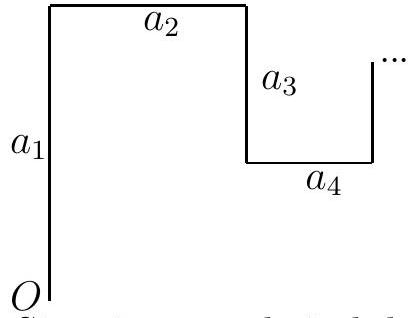
\includegraphics[max width=\textwidth, center]{2024_11_16_1cec5a7f77f0b03e9e54g-5}\\
po nieskończonej łamanej jak na rysunku obok, - $P \quad$ której długości kolejnych odcinków tworzą ciąg geometryczny malejący. Po pewnym czasie cząstka zatrzymała się w punkcie $P(10,3)$. Jaką drogę przebyła cząstka?
  \item Stosując zasadę indukcji matematycznej udowodnić, że dla wszystkich $n \geqslant 1$ wielomian $x^{3 n+1}+x^{3 n-1}+1$ dzieli się bez reszty przez wielomian $x^{2}+x+1$.
  \item Nie przeprowadzając badania przebiegu wykonać wykres funkcji
\end{enumerate}

$$
f(x)=\frac{|x-2|}{x-|x|+2}
$$

Podać równania asymptot i ekstrema lokalne tej funkcji.\\
7. Rozwiązać nierówność

$$
|\cos x|^{1+\sqrt{2} \sin x+\sqrt{2} \cos x} \leqslant 1, \quad x \in[-\pi, \pi] .
$$

\begin{enumerate}
  \setcounter{enumi}{7}
  \item W stożek wpisano graniastosłup trójkątny prawidłowy o wszystkich krawędziach tej samej długości. Przy jakim kącie rozwarcia stożka stosunek objętości graniastosłupa do objętości stożka jest największy?
\end{enumerate}

\section*{PRACA KONTROLNA nr 6}
\begin{enumerate}
  \item W koło o powierzchni $\frac{5}{4} \pi$ wpisano trójkąt prostokątny o polu 1 . Obliczyć obwód tego trójkąta.
  \item Sprowadzić do najprostszej postaci wyrażenie
\end{enumerate}

$$
2\left(\sin ^{6} \alpha+\cos ^{6} \alpha\right)-7\left(\sin ^{4} \alpha+\cos ^{4} \alpha\right)+\cos 4 \alpha
$$

\begin{enumerate}
  \setcounter{enumi}{2}
  \item Wyznaczyć trójmian kwadratowy, którego wykresem jest parabola styczna do prostej $y=x+2$, przechodząca przez punkt $P(-2,-2)$ oraz symetryczna względem prostej $x=1$. Sporządzić rysunek.
  \item W trapezie $A B C D$, w którym $\overline{A B} \| \overline{C D}$, dane są $\overrightarrow{A C}=(4,7)$ oraz $\overrightarrow{B D}=(-6,2)$. Posługując się rachunkiem wektorowym wyznaczyć wektory $\overrightarrow{A B}$ i $\overrightarrow{C D}$, jeśli $\overrightarrow{A D} \perp \overrightarrow{B D}$.
  \item Jaś ma w portmonetce 3 monety jednozłotowe, 2 monety dwuzłotowe i jedną pięciozłotową. Kupując zeszyt w cenie 4 zł wyciąga losowo z portmonetki po jednej monecie tak długo, aż nazbiera się suma wystarczająca do zapłaty za zeszyt. Obliczyć prawdopodobieństwo, że wyciągnie co najmniej trzy monety. Podać odpowiednie uzasadnienie (nie jest nim tzw. drzewko).
  \item Narysować na płaszczyźnie zbiór punktów określony następująco
\end{enumerate}

$$
\mathcal{F}=\left\{(x, y): \sqrt{4 x-x^{2}} \leqslant y \leqslant 4-\sqrt{1-2 x+x^{2}}\right\}
$$

W jakiej odległości od brzegu figury $\mathcal{F}$ znajduje się punkt $P\left(\frac{3}{2}, \frac{5}{2}\right)$ ?\\
7. Dana jest funkcja $f(x)=\log _{2}\left(1-x^{2}\right)-\log _{2}\left(x^{2}-x\right)$. Nie korzystając z metod rachunku różniczkowego wykazać, że $f$ jest rosnąca w swojej dziedzinie oraz, że $g(x)=f\left(x-\frac{1}{2}\right)$ jest nieparzysta. Wyznaczyć funkcję odwrotną $f^{-1}$, jej dziedzinę i zbiór wartości.\\
8. Pole powierzchni bocznej ostrosłupa prawidłowego czworokątnego wynosi $c^{2}$, a kąt nachylenia ściany bocznej do podstawy ma miarę $\alpha$. Ostrosłup rozcięto na dwie części płaszczyzną przechodzącą przez jeden z wierzchołków podstawy i prostopadłą do przeciwległej krawędzi bocznej. Obliczyć objętość części zawierającej wierzchołek ostrosłupa. Kiedy zadanie ma sens?

\section*{PRACA KONTROLNA nr 7}
\begin{enumerate}
  \item Pierwsze dwa wyrazy ciągu geometrycznego są rozwiązaniami równania $4 x^{2}-4 p x-3 p^{2}=0$, gdzie $p$ jest nieznaną liczbą. Wyznaczyć ten ciąg, jeśli suma wszystkich jego wyrazów wynosi 3.
  \item Wiedząc, że $\cos \varphi=\sqrt{\frac{2}{3}}$ oraz $\varphi \in\left(\frac{3}{2} \pi, 2 \pi\right)$, obliczyć cosinus kąta pomiędzy prostymi $y=\left(\sin \frac{\varphi}{2}\right) x, \quad y=\left(\cos \frac{\varphi}{2}\right) x$.
  \item Kostka sześcienna ma krawędź $2 a$. Aby zmieścić ją w pojemniku w kształcie kuli o średnicy $3 a$, ze wszystkich naroży odcięto w minimalny sposób jednakowe ostrosłupy prawidłowe trójkątne. Obliczyć długość krawędzi bocznej odciętych czworościanów?
  \item Udowodnić prawdziwość nierówności
\end{enumerate}

$$
1+\frac{x}{2} \geqslant \sqrt{1+x} \geqslant 1+\frac{x}{2}-\frac{x^{2}}{2} \text { dla } x \in[-1,1]
$$

Zilustrować ją na odpowiednim wykresie.\\
5. Rozwiązać równanie:

$$
\frac{\cos 5 x}{\sin 2 x}=-\sin 3 x
$$

\begin{enumerate}
  \setcounter{enumi}{5}
  \item Znaleźć równanie okręgu symetrycznego do okręgu $x^{2}-4 x+y^{2}+6 y=0$ względem stycznej do tego okręgu poprowadzonej z punktu $P(3,5)$ i majacej dodatni współczynnik kierunkowy.
  \item W okrąg o promieniu $r$ wpisano trapez o przekątnej $d \geqslant r \sqrt{3}$ i największym obwodzie. Obliczyć pole tego trapezu.
  \item Metodą analityczną określić dla jakich wartości parametru $m$ układ równań
\end{enumerate}

$$
\left\{\begin{array}{rr}
m x & -y+2=0 \\
x & -2|y|+2=0
\end{array}\right.
$$

ma dokładnie jedno rozwiązanie? Wyznaczyć to rozwiązanie w zależności od $m$. Sporządzić rysunek.


\end{document}